\section{Introduction}
% background and context, can get this from thesis and safety document

The CERN High Energy Accelerator Mixed-field (\href{http://charm.web.cern.ch/CHARM/}{CHARM}) facility is situated in the Proton Synchrotron (PS) East Area hall at the Meyrin Site of CERN in Switzerland. A map in figure \ref{fig:meyrin_map} shows the location on the Meyrin site, and a 3D rendered image of the East Area hall is shown in figure \ref{fig:eastarea_hall_3d}. The aim of the CHARM facility is to have a flexible and dedicated place for the testing of electronics and systems in well characterised mixed-radiation fields, which can replicate a wide number of real radiation environments such as space, atmosphere, or accelerator complexes for example. To achieve this, the test area has been constructed with the sole purpose of flexibility in electronics testing. \\

Starting with the 24 GeV proton beam from the PS, the beam is directed along a number of beam-lines to various physics experiments. The CHARM facility is located at the end of the T8 beam-line in the PS East Area Hall. The T8 beam-line is shared with the IRRAD facility, located up-stream of CHARM. Once the beam passes through IRRAD, it enters the CHARM test area where it impinges on 1 of the 3 possible targets (and alternatively without target). Depending on the target selection, the radiation field can be varied inside the test area. Additionally, there are 4 movable shielding layers of iron and concrete inside the test area which can further alter the radiation field. Finally there are a number of dedicated test positions around the test area, which are selected based on the radiation field requirements of the user. \\
 
To understand the radiation field within the test area, dedicated FLUKA \cite{FLUKA1} \cite{FLUKA2} Monte Carlo calculations have been made for the various facility configurations and test positions. Using these results, one can describe the radiation spectra seen at each test position and calculate useful quantities related to electronics testing, such as the total ionising dose (TID) or 1 MeV equiverlent neutron fluence in Silicon for example. A detailed list of the available information is shown in chapter 3. These values can then be used to calculate failure rates and tolerances of test equipment to be installed and used in environments where radiation is present. \\

\begin{figure}[!ht]
	\centering
	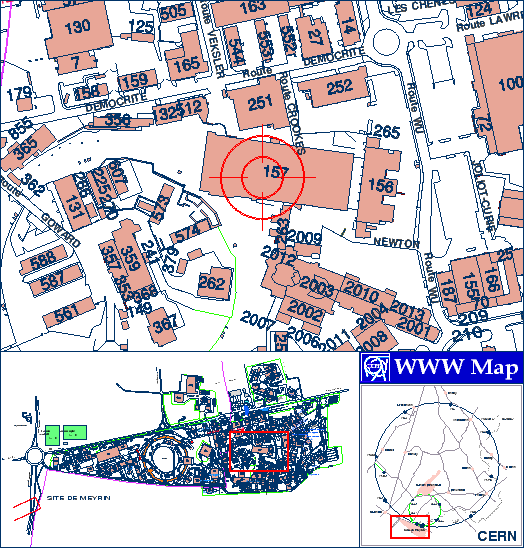
\includegraphics[width=0.6\textwidth]{./images/meyrin_map_157}
	\caption{A map of the CERN Meyrin site showing the location of building 157, where the IRRAD and CHARM facility are located (\url{http://building.web.cern.ch/building/})}
	\label{fig:meyrin_map}
\end{figure}

\begin{figure}[!ht]
	\centering
	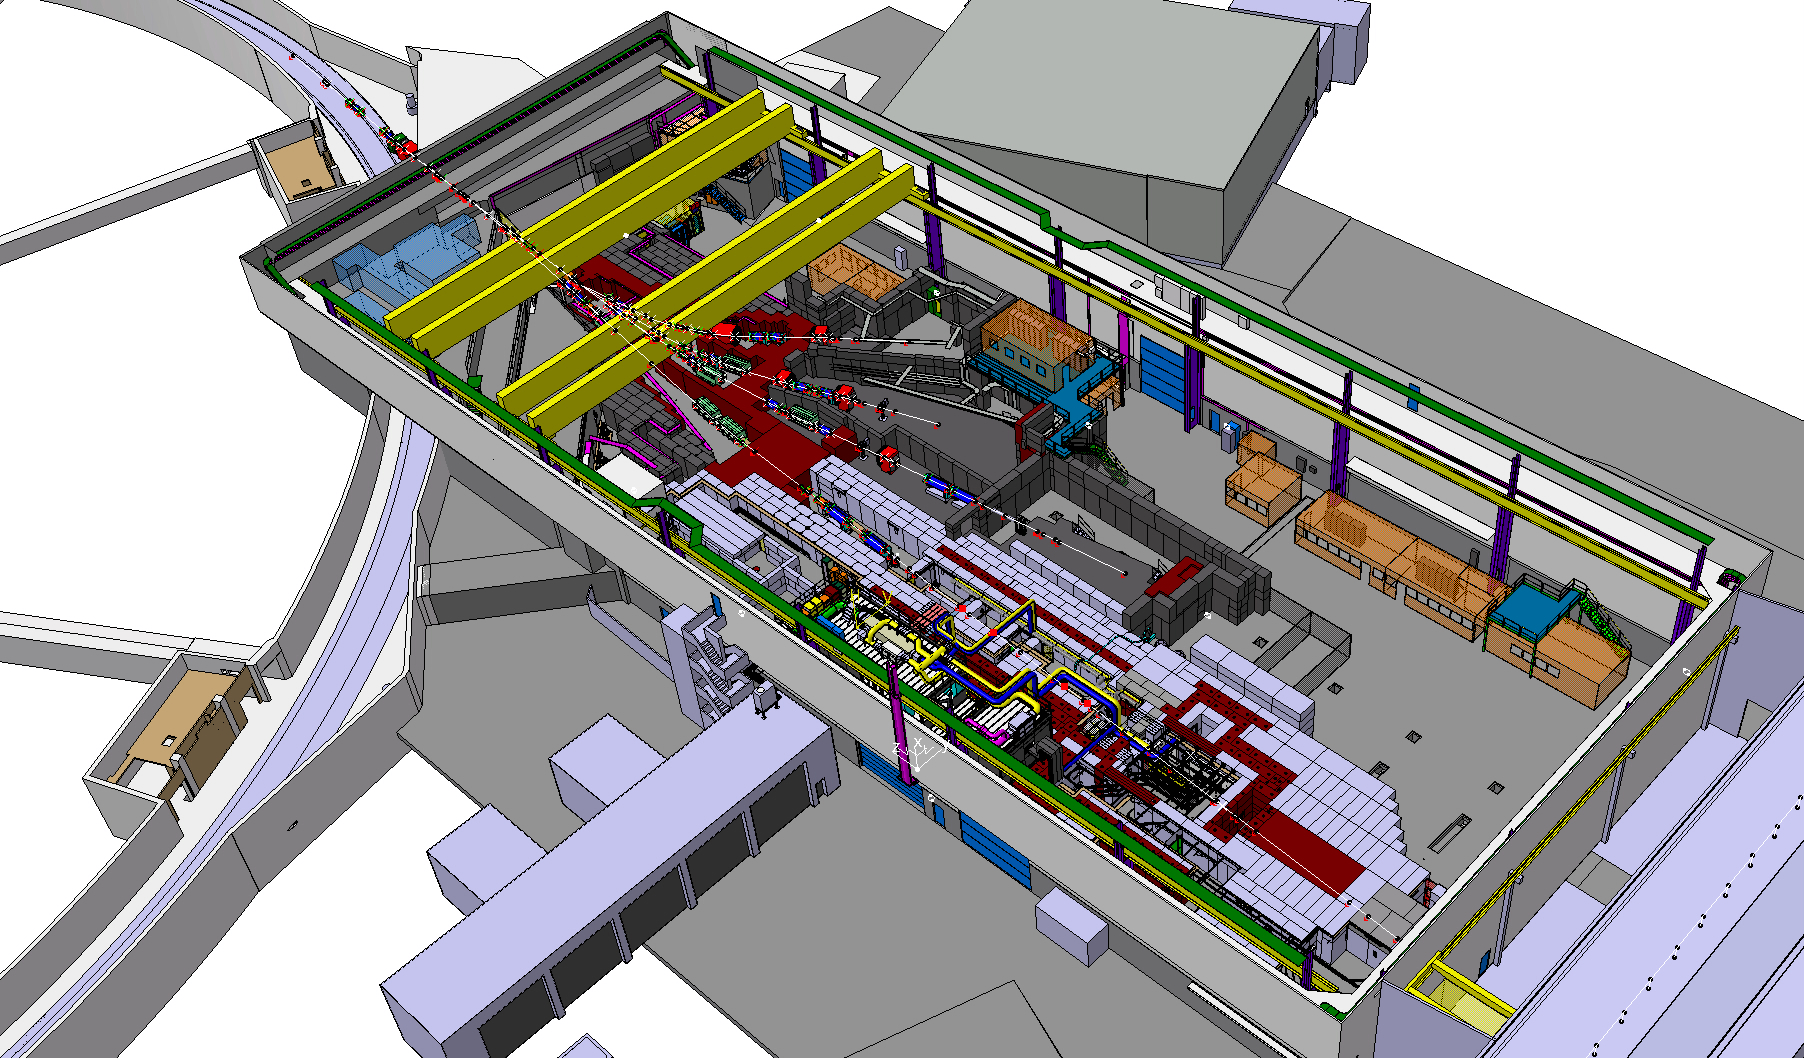
\includegraphics[width=0.9\textwidth]{./images/EastArea-Vue3D-1}
	\caption{A screen-shot from the 3D drawing of the PS East Area Hall. The IRRAD and CHARM facility are located in the southern part of the hall (bottom-right of the image).}
	\label{fig:eastarea_hall_3d}
\end{figure}